\documentclass[a4paper,11pt]{ujreport}
%%【PostScript, JPEG, PNG等の画像の貼り込み】
%% 利用するパッケージを選んでコメントアウトしてください.
\usepackage{graphicx} % for \includegraphics[width=3cm]{sample.eps}
\usepackage{epsfig} % for \psfig{file=sample.eps,width=3cm}
%\usepackage{epsf} % for \epsfile{file=sample.eps,scale=0.6}
%\usepackage{epsbox} % for \epsfile{file=sample.eps,scale=0.6}
\usepackage{src/class/mediabb} % for pdf

\usepackage{times} % use Times Font instead of Computer Modern
% \usepackage{listings} % for soursecode
% \usepackage{plistings} % for soursecode
\usepackage{src/class/docmute} % texファイル分割用

\setcounter{tocdepth}{3}
\setcounter{page}{-1}

\setlength{\oddsidemargin}{0.1in}
\setlength{\evensidemargin}{0.1in}
\setlength{\topmargin}{0in}
\setlength{\textwidth}{6in}
%\setlength{\textheight}{10.1in}
\setlength{\parskip}{0em}
\setlength{\topsep}{0em}

%\newcommand{\zu}[1]{{\gt \bf 図\ref{#1}}}

%% タイトル生成用パッケージ(重要)
\usepackage{src/class/mast-jp-sjis}

%% タイトル
%% 【注意】タイトルの最後に\\ を入れるとエラーになります
\title{NoSQL型データベースシステムでの実体化ビュー選択に関する研究}
%% 著者
\author{髙木 颯汰}
%% 指導教員
\advisor{古瀬 一隆 陳 漢雄}

%% 年月 (提出年月)
%% 年月は必要に応じて書き替えてください.
\majorfield{ } \yearandmonth{2019年 1月}


\addtocounter{page}{2} %単体でコンパイルした際の調整用
\begin{document}

\chapter{実験}
\label{chap:Experiment}
\section{Mongooseについて}
MongooseとはMongoDB用モデリングツールで,Node.jsの非同期環境でうまく動作することを目的として設計されている.Mongooseを使用すれば,モデルを定義して操作することで,MongoDBのコレクション/ドキュメントを操作できる\cite{mongoose}.本論文ではMongooseを用いてMongoDBを操作するミドルウェアを実装する.

\section{実験環境}
実験環境に関する情報を表\ref{table:experiment_env}に示す.
\begin{table}[htb]
  \begin{center}
    \caption{実験環境}
		\label{table:experiment_env}
    \begin{tabular}{|c|c|} \hline
      マシン & MacBook (Retina, 12-inch, 2017) \\ \hline
      プロセッサ & 1.2 GHz Intel Core m3\\ \hline
      メモリ & 8 GB 1867 MHz LPDDR3\\ \hline
      データベースシステム & Mongodb version 3.1.10\\ \hline
    \end{tabular}
  \end{center}
\end{table}

\section{実験方法}
本論文の実験で用いたコレクションはpersonコレクション,storyコレクション,commentコレクション,publisherコレクションである.コレクションの構造,コレクション同士の参照に関しては図\ref{ExperimentCollection},図\ref{ExperimentCollection2}に示す.storyコレクションには筆者として1つのpersonドキュメントのidを格納する.このstoryドキュメントが検索された際には筆者のidをperosnコレクションから検索し,結合して結果を返す.同じようにファンとしてpersonドキュメントのidを配列で格納することで複数のpersonドキュメントをstoryドキュメントに埋め込む.実際の実験データではファンとして100のpersonドキュメントのidを埋め込む.その際,100回結合処理を実行することになる.出版社としてpublisherドキュメントのidも格納する.
\begin{figure}[htbp]
	\begin{center}
		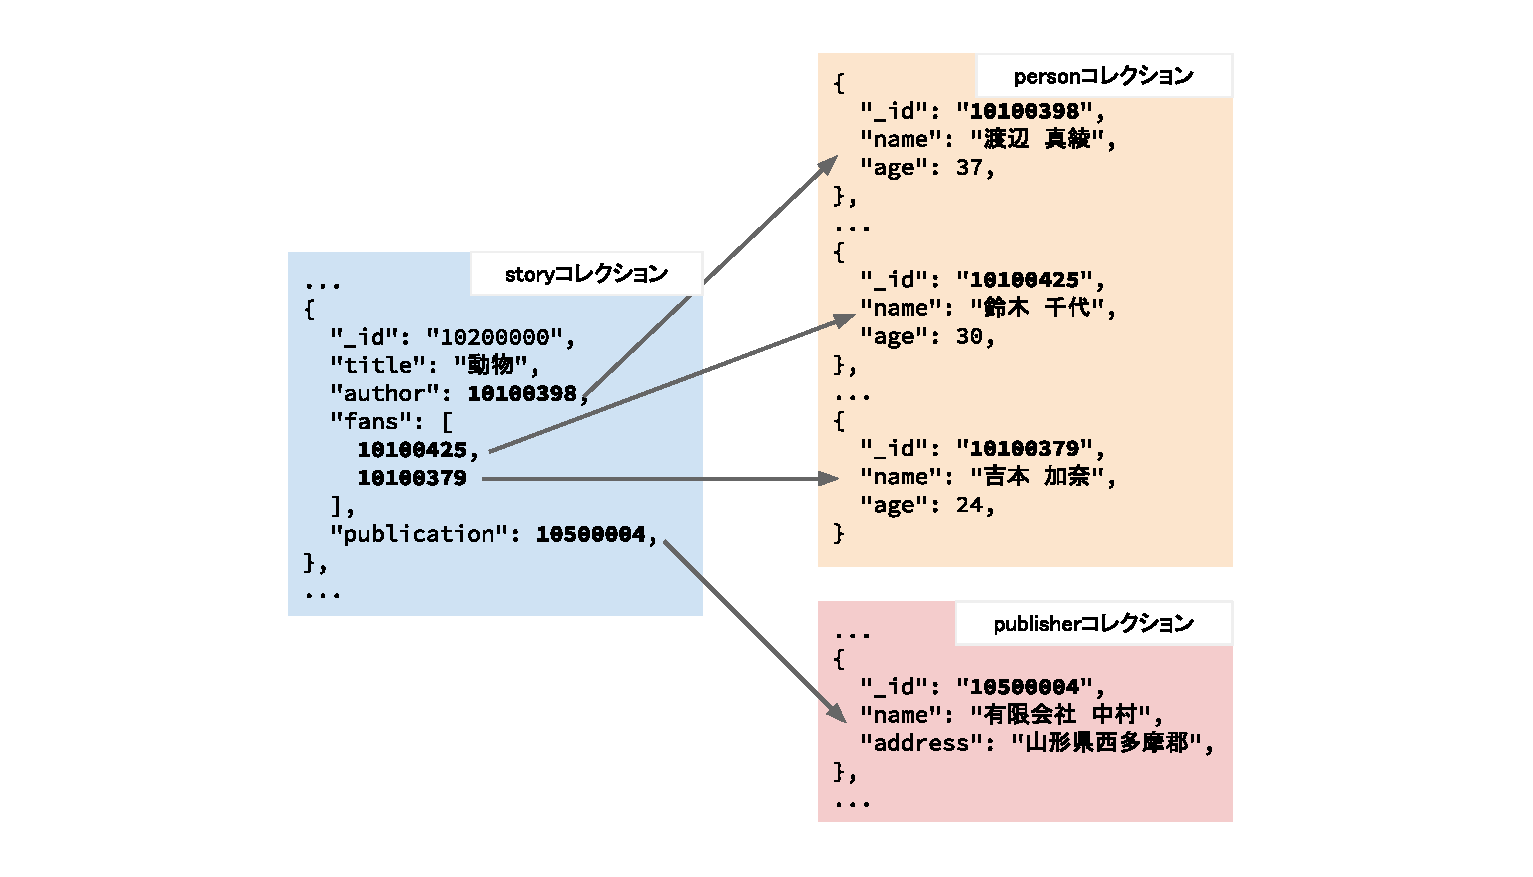
\includegraphics[width=30em, trim=10em 2em 10em 2em]{/Users/takagihayata/workspace/materialize-mongodb/paper/mast/src/ExperimentCollection.eps} %[trim=left bottom right top]
	\end{center}
	\caption{storyコレクションから各コレクションへの参照}
	\label{ExperimentCollection}
\end{figure}
\begin{figure}[htbp]
	\begin{center}
		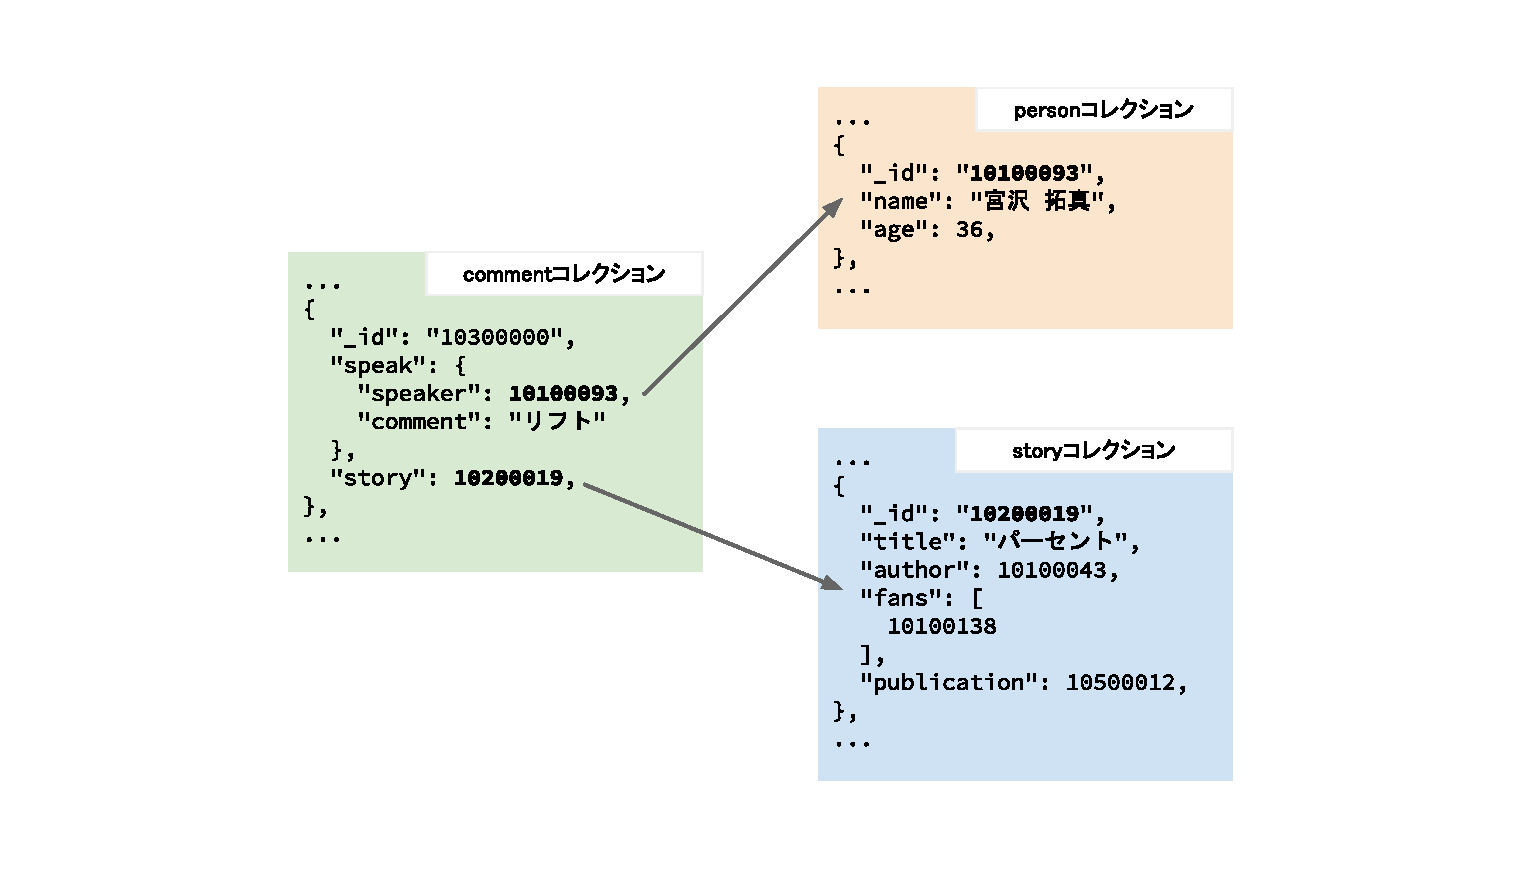
\includegraphics[width=30em, trim=10em 2em 10em 2em]{/Users/takagihayata/workspace/materialize-mongodb/paper/mast/src/ExperimentCollection2.eps} %[trim=left bottom right top]
	\end{center}
	\caption{commentコレクションから各コレクションへの参照}
	\label{ExperimentCollection2}
\end{figure}
実験において使用するデータは全て参照型のデータモデルで挿入する.実体化していない状態で検索された場合には結合処理を行い結果を返す.実験に用いるドキュメントはPythonのライブラリであるfaker\cite{faker}を用いて作成した.各コレクションに対して1000ドキュメントを作成した.


実験では全てのコレクションが従来の参照型のデータモデルを用いたシステムと実体化条件を用いずに全てのコレクションを実体化したシステム,実体化条件を用いて適宜コレクションを実体化するシステムの3つのデータベースシステムを比較する.その際,実体化を用いたシステムでは検索や更新を提案ミドルウェアを用いて処理する.

この3つのシステムを比較する際,検索と更新の比率を変えた4つのクエリパターンを用いて行う.このクエリパターンを表に示す.このパターンを用いて実験A,B,C,Dを行う.
\begin{table}[htb]
  \begin{center}
    \caption{クエリパターン}
		\label{table:experiment_query_pattern}
    \begin{tabular}{|c|c|c|} \hline
        & 検索回数 & 更新回数 \\ \hline
      パターンA & 99 & 1\\ \hline
      パターンB & 97 & 3\\ \hline
			パターンC & 95 & 5\\ \hline
      パターンD & 90 & 10\\ \hline
    \end{tabular}
  \end{center}
\end{table}
それぞれのパターンに対して,使用したクエリを表で示す.ここではMongooseのpopulateを用いて結合処理をおこなっている.また,提案手法を用いる場合には検索・更新に関わらずクエリが5回処理された際に実体化条件を検討し,適宜実体化ビューを作成,破棄を行う.
\begin{table}[htb]
  \begin{center}
    \caption{実験で使用した検索クエリ}
		\label{table:ExperimentFindQuery}
    \begin{tabular}{|c|l|} \hline
      コレクション & \multicolumn{1}{|c|}{クエリ}\\ \hline
      person & db.person.find(\{\_id: testID\})populate([]);\\ \hline
			story & db.story.find(\{\_id: testID\}).populate(["author", "fans", "publication", "comments"]);\\ \hline
      comment & db.comment.find(\{\_id: testID\}).populate(["speak.speaker", "story"]);\\ \hline
      publisher & db.publisher.find(\{\_id: testID\}).populate([]);\\ \hline
    \end{tabular}
  \end{center}
\end{table}
\begin{table}[htb]
  \begin{center}
    \caption{実験で使用した更新クエリ}
		\label{table:ExperimentUpdateQuery}
    \begin{tabular}{|c|l|} \hline
      コレクション & \multicolumn{1}{|c|}{クエリ}\\ \hline
      person & db.person.update(\{\_id: testID\}, \{\$set: \{name: "太郎"\}\});\\ \hline
			story & db.story.update(\{\_id: testID\}, \{\$set: \{title: "研修資料"\}\});\\ \hline
      comment & db.comment.update(\{\_id: testID\}, \{\$set: \{"speak.comment": "いい天気"\}\});\\ \hline
      publisher & db.publisher.update(\{\_id: testID\}, \{\$set: \{address: "つくば市天王台"\}\});\\ \hline
    \end{tabular}
  \end{center}
\end{table}

\end{document}
